\chapter{The ATLAS Detector}
\label{chap:atlas}
The A Toroidal LHC ApparatuS (ATLAS) is the largest general purpose detector at the LHC.  It is designed to record and reconstruct the products of proton proton collisions over a broad range of energies and final state topologies. The detector combines tracking, calorimetry, and muon detection systems in order to provide precise measurements of charged particle trajectories, particle energies, and event level observables. 

ATLAS is built in a cylindrical geometry around the beam axis, with subdetectors arranged in concentric layers. The coordinate system is defined with its origin at the nominal interaction point. The $z$ axis is aligned with the beam direction, the $x$ axis points from the interaction point toward the centre of the LHC ring, and the $y$ axis points upward. In the plane transverse to the beam, particle directions are described by the azimuthal angle $\phi$. The polar angle $\theta$ with respect to the beam axis is commonly expressed in terms of pseudorapidity $\eta = -\ln\tan(\theta/2)$

\begin{figure}[H]
    \centering
    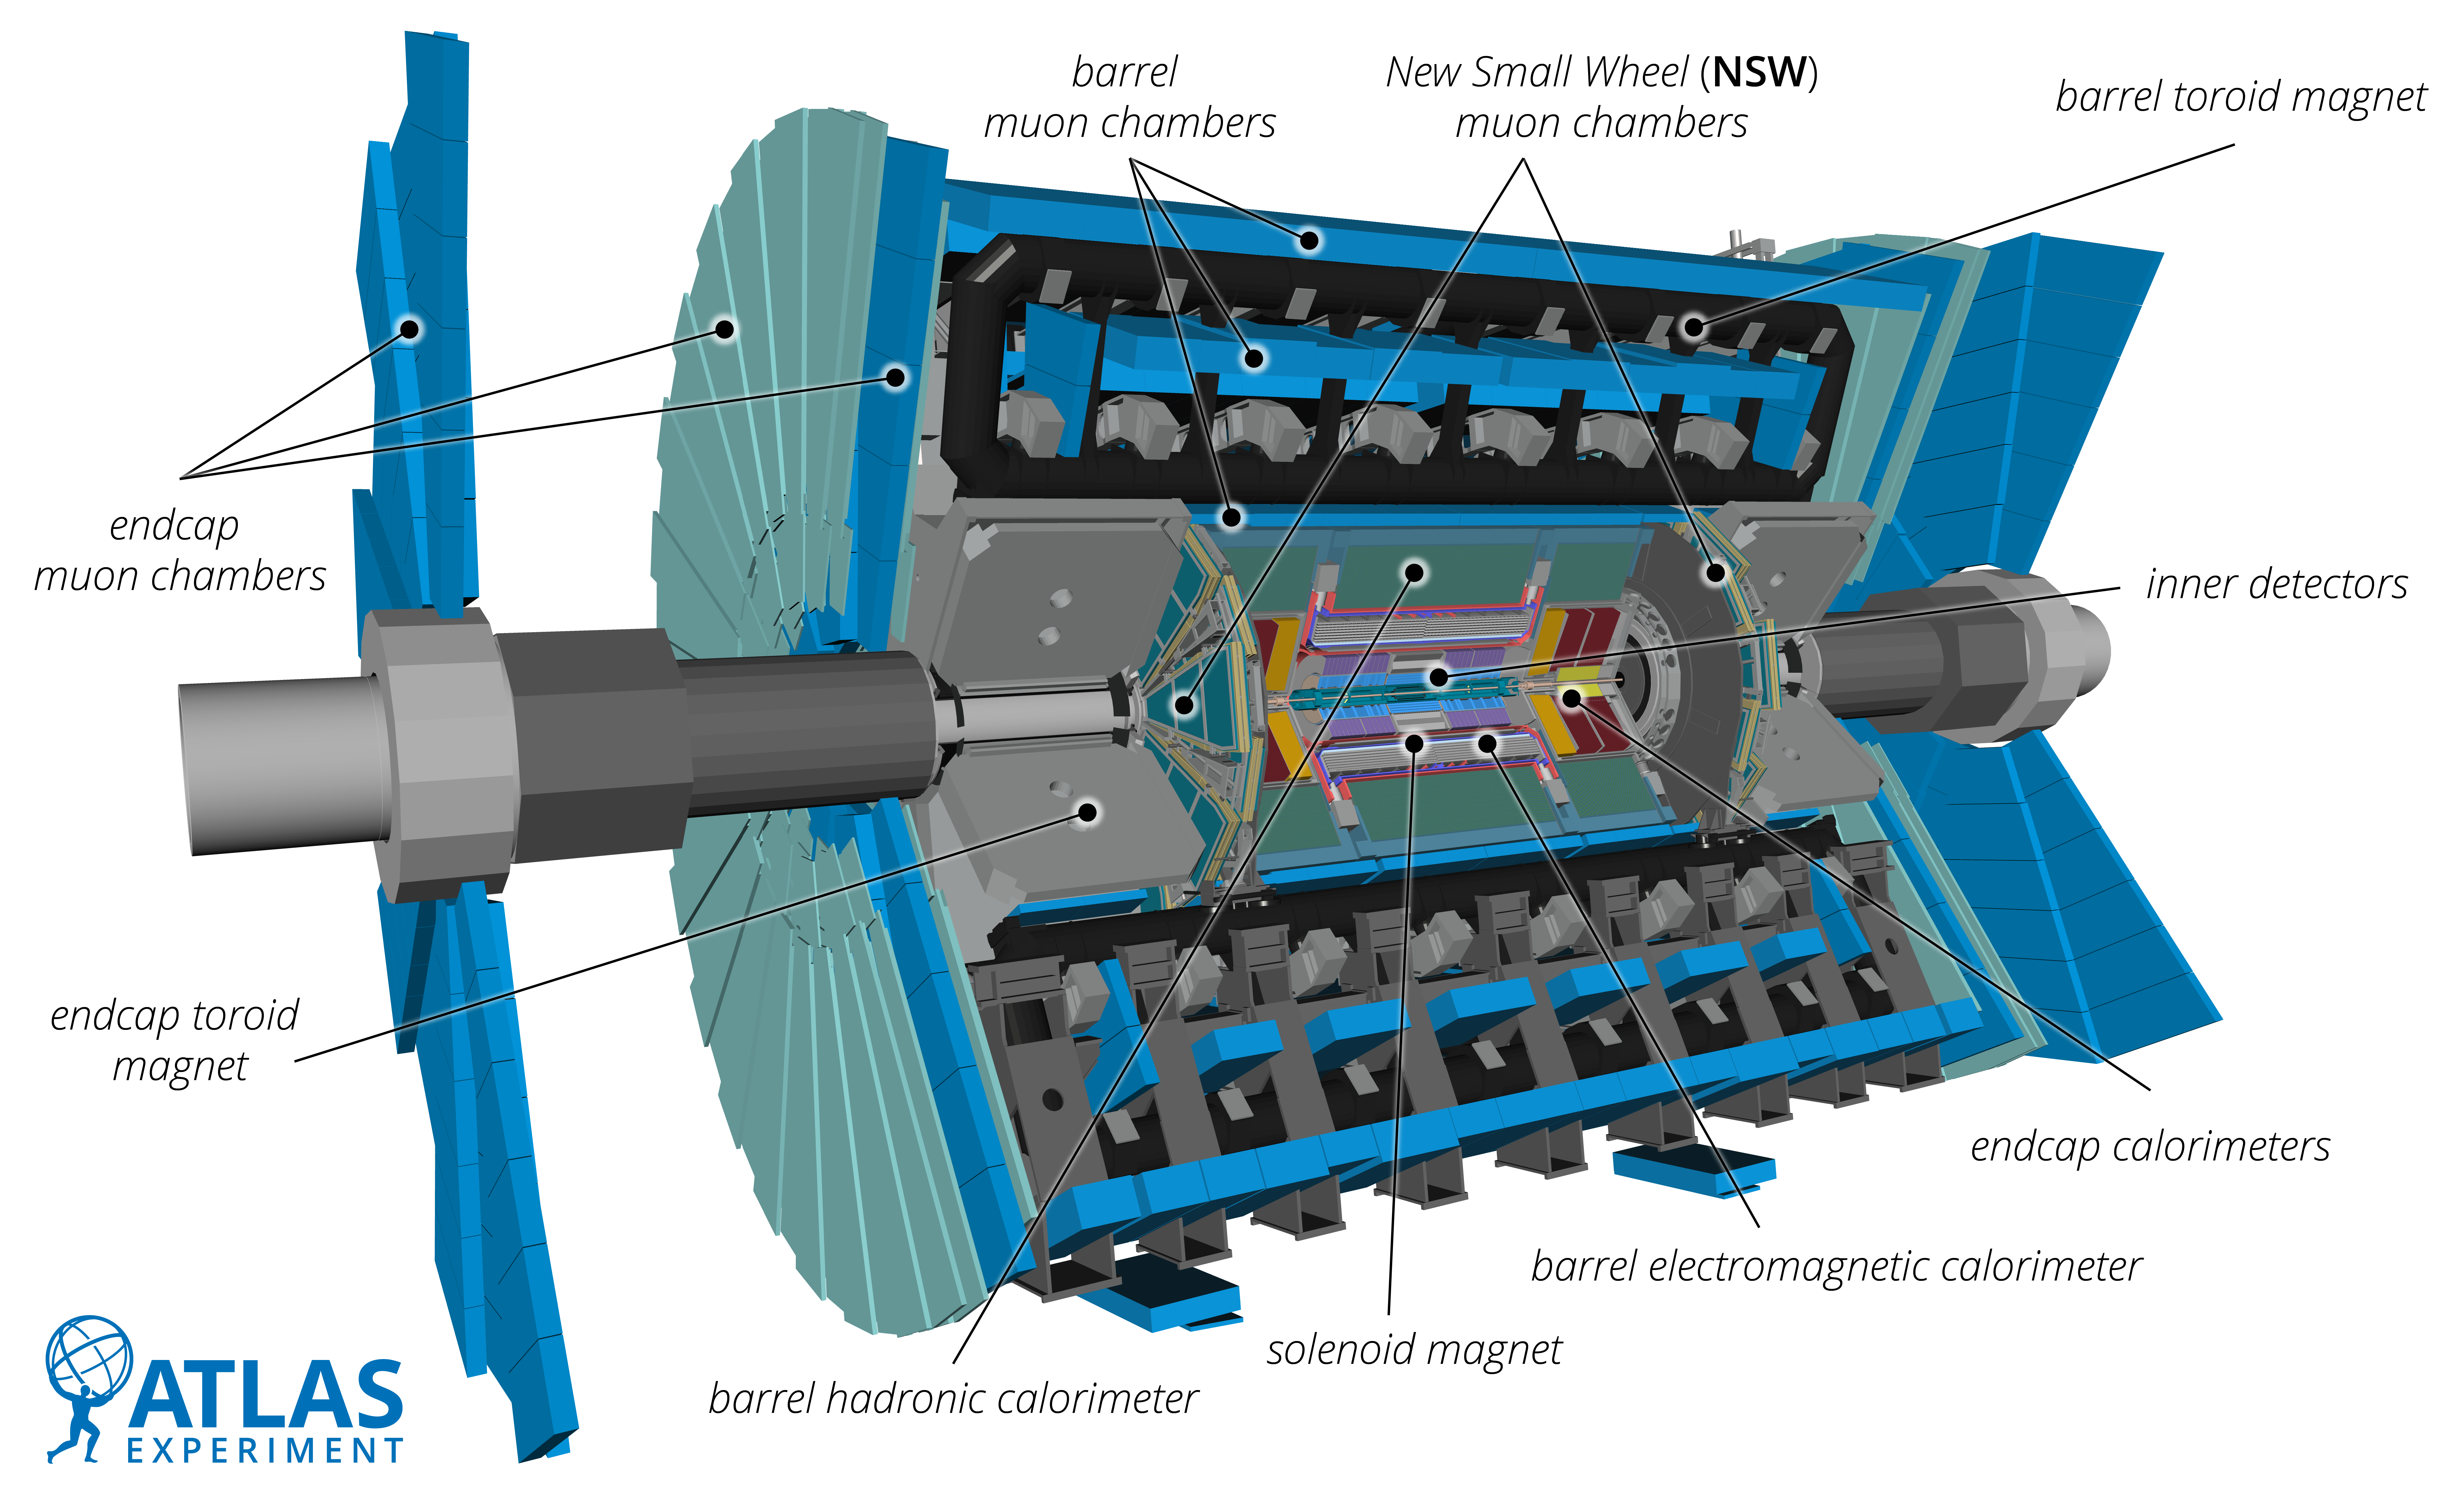
\includegraphics[width=0.95\textwidth]{figures/Detector.png}
    \caption{Schematic view of the ATLAS detector.}
    \label{fig:atlas_detector}
\end{figure}